\documentclass{eeleyes}

\usetikzlibrary{arrows,automata,positioning}

\newtcolorbox{solution}{
	breakable,
	coltitle = black,
	colback = white,
	frame hidden,
	boxrule = 0pt,
	boxsep = 0pt,
	borderline west={2pt}{0pt}{black},
	sharp corners = all,
	enhanced,
}

\begin{document}

\section*{Problem 1}
% \textit{
Construct a DFA that recognizes strings in $\{0, 1\}*$ with the following property. Each string, when interpreted as a binary number, is congruent to $3$ modulo $5$. 
% }

\begin{solution}
    If a number reduces $3 \pmod{5}$, then it must reduce either $3 \pmod{10}$ or $8 \pmod{10}$. Therefore the binary digit representation must end in either a $3 \equiv (10)_2$ or $8 \equiv (1000)_2$. Therefore we make a machine that only accepts strings with either of those endings.

    \begin{center}
        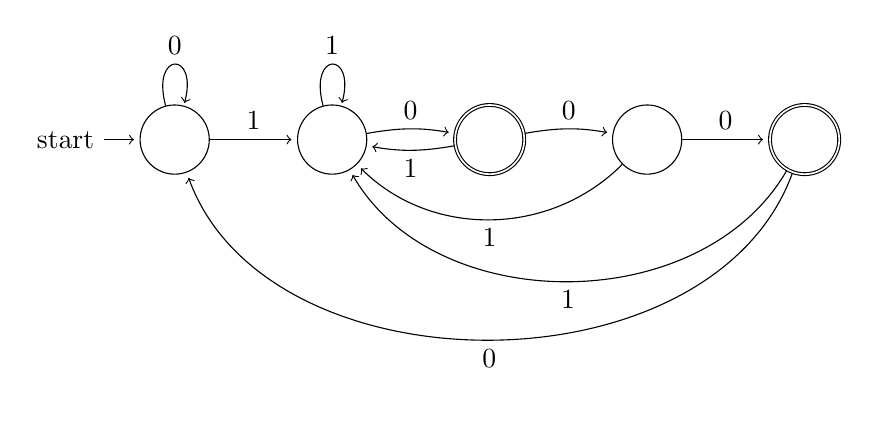
\begin{tikzpicture}[shorten >=2pt,node distance=2cm,on grid,auto]
            \tikzstyle{every state}=[fill=white]

            \node[state, initial]   (s1)               {};
            \node[state]            (s2) [right of=s1] {};
            \node[state, accepting] (s3) [right of=s2] {};
            \node[state]            (s4) [right of=s3] {};
            \node[state, accepting] (s5) [right of=s4] {};

            \path[->]
                (s1) edge node {$1$} (s2)
                (s1) edge [loop above] node {$0$} (s1)

                (s2) edge [loop above] node {$1$} (s2)
                (s2) edge [bend left=10] node {$0$} (s3)

                (s3) edge [bend left=10] node {$0$} (s4)
                (s3) edge [bend left=10] node {$1$} (s2)

                (s4) edge node {$0$} (s5)
                (s4) edge [bend left=45] node {$1$} (s2)

                (s5) edge [bend left=60] node {$1$} (s2)
                (s5) edge [bend left=70] node {$0$} (s1)
                ;
        \end{tikzpicture}
    \end{center}
\end{solution}

\section*{Problem 2}
Design a DFA over the alphabet $\Sigma = \{a, b\}$ that accepts all strings with an even number of instances of the letter $a$ and an odd number of instances of the letter $b$.

\begin{solution}
    We create a state for each possible pair of parities of $a$ and $b$ and appropriately transition between them.

    \begin{center}
        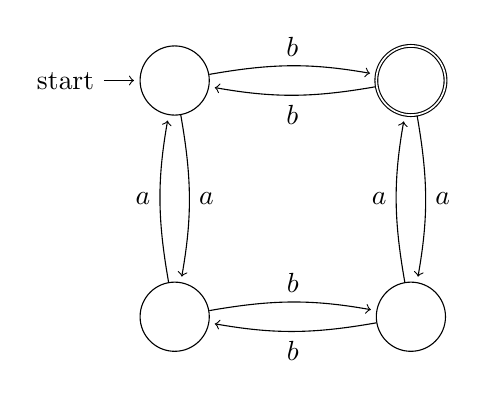
\begin{tikzpicture}[shorten >=2pt,node distance=3cm,on grid,auto]
            \tikzstyle{every state}=[fill=white]

            \node[state, initial]   (ee)               {};
            \node[state, accepting] (eo) [right of=ee] {};
            \node[state]            (oe) [below of=ee] {};
            \node[state]            (oo) [right of=oe] {};

            \path[->]
                    (ee) edge [bend left=10] node {$a$} (oe)
                    (ee) edge [bend left=10] node {$b$} (eo)

                    (eo) edge [bend left=10] node {$a$} (oo)
                    (eo) edge [bend left=10] node {$b$} (ee)

                    (oe) edge [bend left=10] node {$a$} (ee)
                    (oe) edge [bend left=10] node {$b$} (oo)

                    (oo) edge [bend left=10] node {$a$} (eo)
                    (oo) edge [bend left=10] node {$b$} (oe)
                ;
        \end{tikzpicture}
    \end{center}
\end{solution}


\section*{Problem 3}
Give a simple English description of the language recognized by the following machine
\begin{center}
    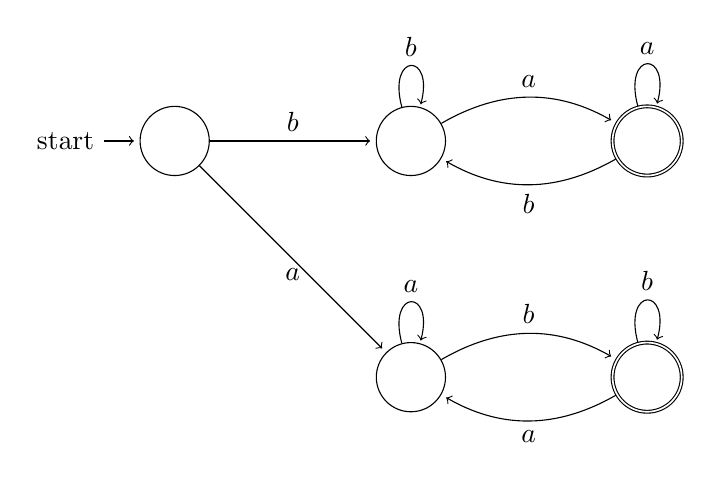
\begin{tikzpicture}[shorten >=2pt,node distance=3cm,on grid,auto]
        \tikzstyle{every state}=[fill=white]

        \node[state, initial]   (s0) {};
        \node[state]            (t0) [right of=s0] {};
        \node[state, accepting] (t1) [right of=t0] {};

        \node[state]            (b0) [below of=t0] {};
        \node[state, accepting] (b1) [below of=t1] {};

        \path[->] 
            (s0) edge              node              {$b$} (t0)
            (s0) edge              node [below]      {$a$} (b0)

            (t0) edge [loop above] node              {$b$}
            (t0) edge [bend left]  node              {$a$} (t1)

            (t1) edge [loop above] node              {$a$}
            (t1) edge [bend left]  node              {$b$} (t0)

            (b0) edge [loop above] node              {$a$}
            (b0) edge [bend left]  node              {$b$} (b1)

            (b1) edge [loop above] node              {$b$}
            (b1) edge [bend left]  node              {$a$} (b0)
        ;
    \end{tikzpicture}
\end{center}

\begin{solution}
    The machine recognizes strings whose starting and ending letters are different.
\end{solution}

\section*{Problem 4}
Give a simple English description of the language recognized by the following NFA
\begin{center}
    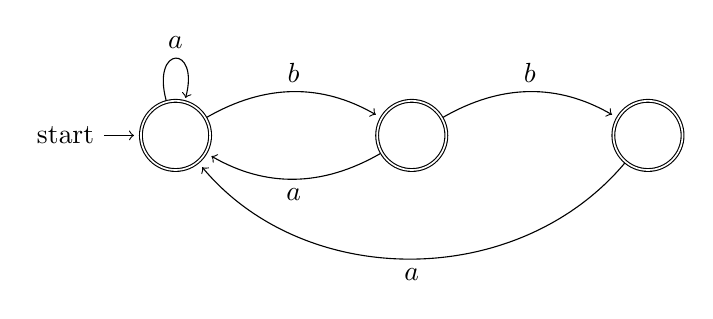
\begin{tikzpicture}[shorten >=2pt,node distance=3cm,on grid,auto]
        \tikzstyle{every state}=[fill=white]

        \node[state, initial, accepting]   (s0)               {};
        \node[state, accepting]            (s1) [right of=s0] {};
        \node[state, accepting]            (s2) [right of=s1] {};

        \path[->] 
            (s0) edge [loop above] node              {$a$} (s0)
            (s0) edge [bend left ] node              {$b$} (s1)

            (s1) edge [bend left ] node              {$a$} (s0)
            (s1) edge [bend left ] node              {$b$} (s2)

            (s2) edge [bend left=50] node              {$a$} (s0)
        ;
    \end{tikzpicture}
\end{center}

\begin{solution}
    The machine recognizes strings that dont contain a substring of b's more than $2$ letters long.
\end{solution}

\end{document}
